%!TEX root = ../report.tex
\section{Risk assessment}
The system is confronted by severals risks which are determined and mitigated in this section.

%Risk impact assesment and Prioritization
% Probability of Occurrence ( In the appendice is the table to which show how to evaluate a risk and the severity of consequences 
%http://www.mitre.org/publications/systems-engineering-guide/acquisition-systems-engineering/risk-management/risk-impact-assessment-and-prioritization %)

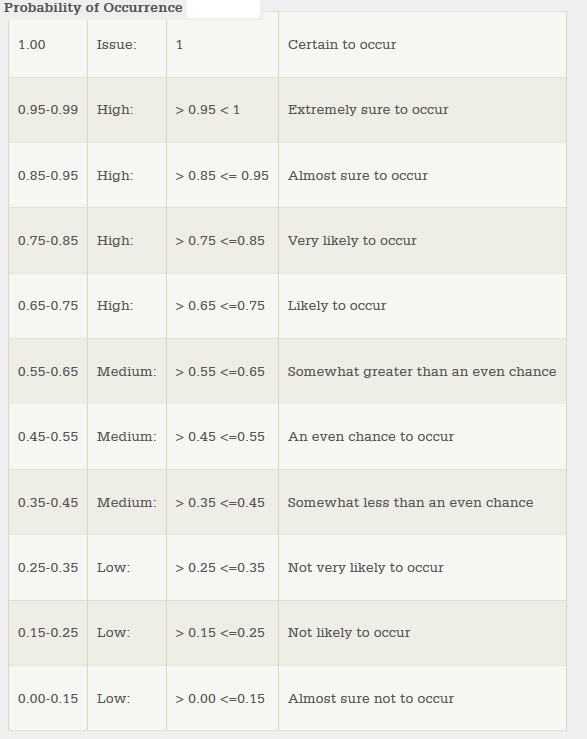
\includegraphics[scale=0.5]{C:/Users/admin/Desktop/M1/RISKSOCCURENCE.jpg} % maybe in the appendice ?
\subsection{Techincal}

\begin{longtable}{L{0.1\textwidth} L{0.0\textwidth} L{0.7\textwidth}}
	\textbf{Nr.} &  & \textbf{Description} \\
	\reqRow{risk}{1}{}{The warning system does not detect floods in time}  \\ 
	%{}Probability of Occurence : Low \\ 
	%Timeframe
	%{}Consequences : Severe }
	%Decision
	\reqRow{risk}{2}{}{The system sends warnings of a non-excising flood (false positive), making people more negligent to future messages.}
	% Probability of Occurence : LOW
	%Timeframe
	%Consequences
	%Decision
	\reqRow{risk}{3}{}{The system can't send messages to the necessary people because the communication platform is also destroyed by the flood.}
	%Probability of Occurence :MEDIUM
	%Timeframe
	%Consequences
	%Decision
	\reqRow{risk}{4}{}{The system sends incorrect information, causing extra damage.}
	%Probability of Occurence :LOW
	%Timeframe
	%Consequences
	%Decision
	\reqRow{risk}{5}{}{Hacker get access to the system} % is this riskworthy?
	%Probability of Occurence :LOW
	%Timeframe
	%Consequences
	%Decision

	\bottomrule
\end{longtable}



%\begin{tabular} {l | c | r }
%Risk & Consequence & Solution \\
%\end{tabular}

\subsection{Business}


\begin{longtable}{L{0.1\textwidth} L{0.0\textwidth} L{0.7\textwidth}}
	\textbf{Nr.} &  & \textbf{Description} \\
	\reqRow{risk}{1}{}{Wrong estimation of the budget}
	%Probability of Occurence :Medium
	%Timeframe
	%Consequences
	%Decision
	\reqRow{risk}{2}{}{The money invested in the fabrication of the system isn't "covered" by the sells (shortfall/deficit)}
	%Probability of Occurence :Medium
	%Timeframe
	%Consequences
	%Decision
	\reqRow{risk}{3}{}{Competitors lowering their prices so our company has to reduce its} % is this riskworthy?
	%Probability of Occurence : Medium
	%Timeframe
	%Consequences
	%Decision
	\reqRow{risk}{4}{}{The sensors company become bankrupt}
	%Probability of Occurence :Low
	%Timeframe
	%Consequences
	%Decision
	\bottomrule
\end{longtable}




\textit{(HOW TO HANDLE THOSE RISKS ? SCALE OF RISKS , PROBABILITY THAT THOSE RISKS HAPPEN , How to evaluate a risk ? Measurement ?)}


